\chapter*{Introduction}
\begin{figure}[h]
	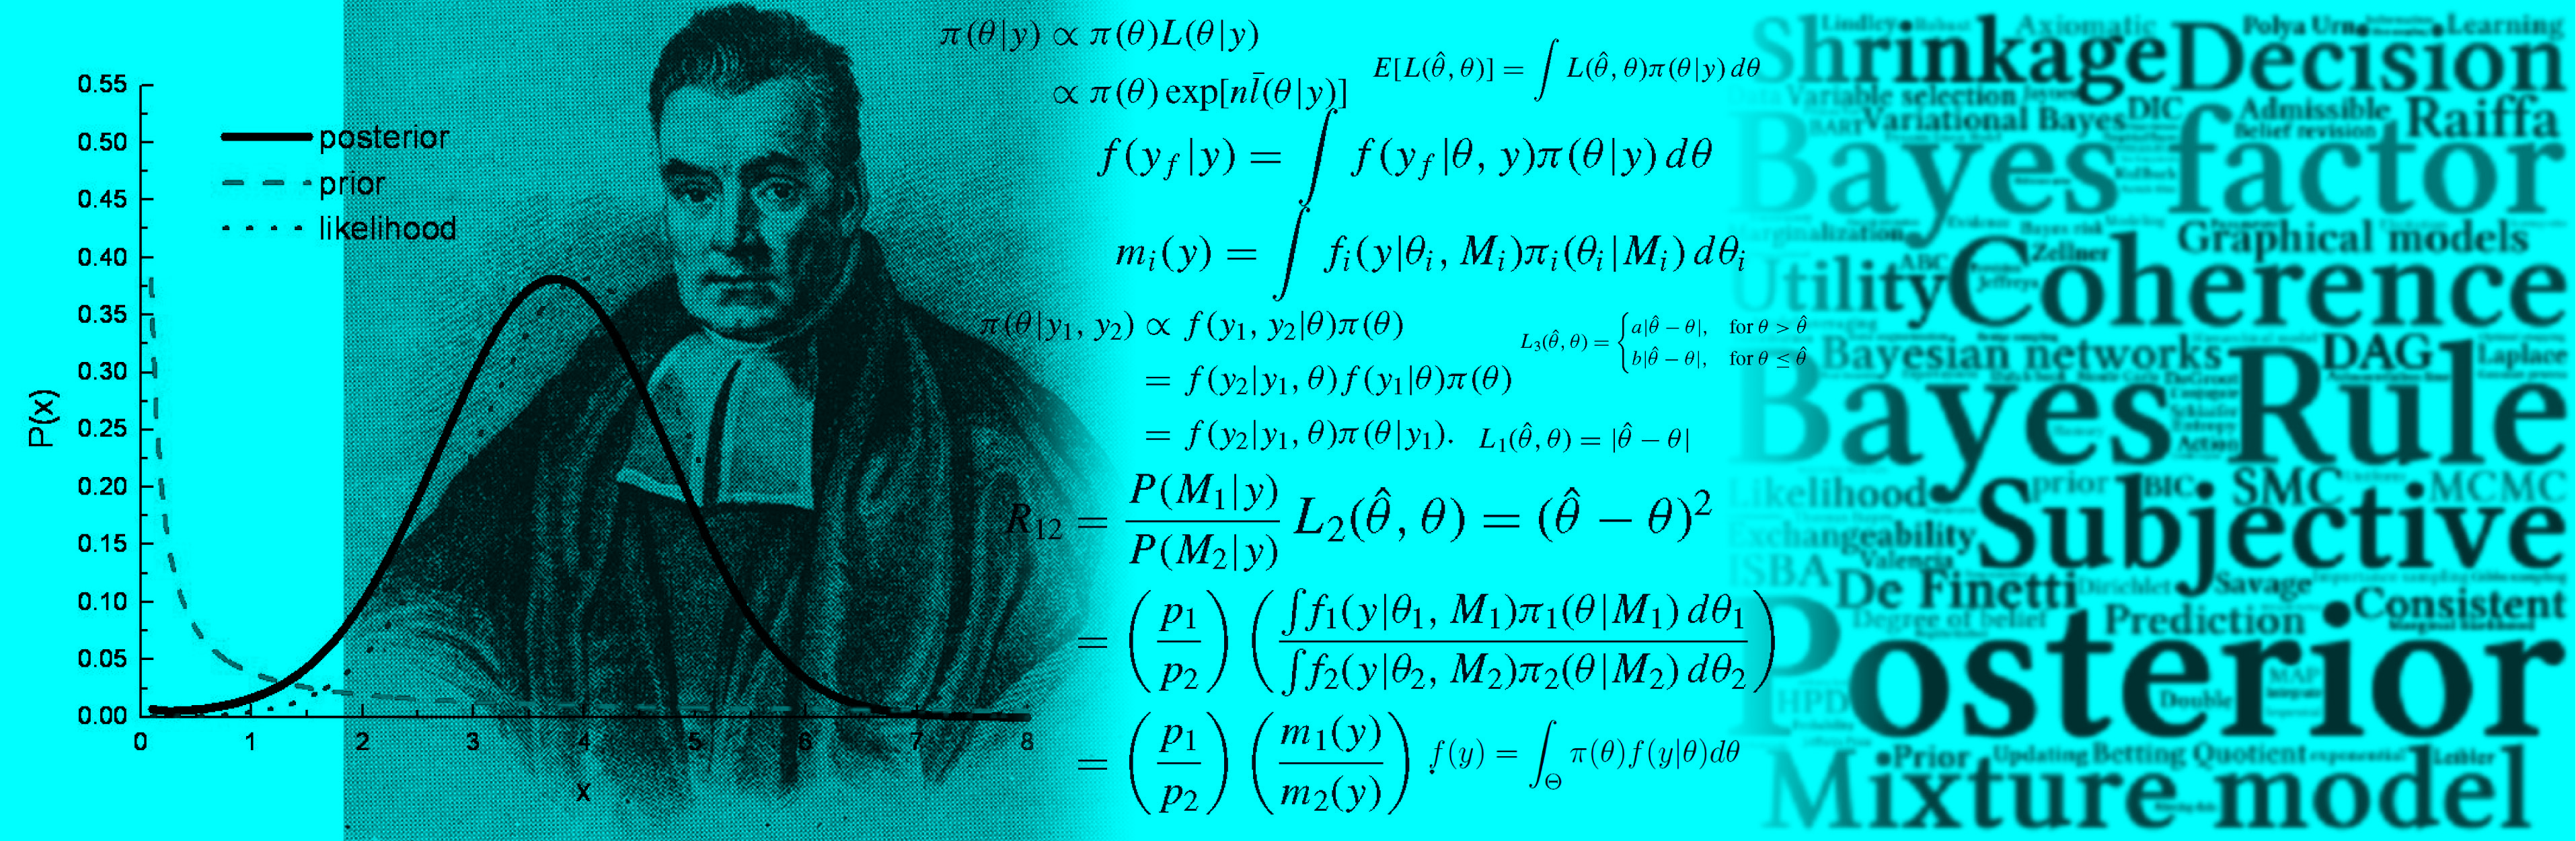
\includegraphics[width=340pt, height=150pt]{frontmatter/figures/BannerBook.jpg}
	%%\centerline{\epsfig{/Chapters/chapter1/figures/cat.eps,width=.8\textheight,height=.4\textwidth}}
	\caption[List of figure caption goes here]{\textit{Supposedly} portrait of Thomas Bayes.}\label{fig01}
\end{figure}

Since late 90’s Bayesian inference has gained a lot of popularity among researchers due to the computational revolution and availability of algorithms to solve complex integrals. However, many researchers, students and practitioners still lack understanding and application of this inferential approach. The main reason is the requirement of good programming skills.

\textbf{Introduction to Bayesian inference: A GUIded tour using R} mainly targets those who want to apply Bayesian regression analysis having a good conceptual and formal understanding, but not having time to develop programming skills. Thus, this book provides a graphical user interface (GUI) to carry out Bayesian regression in a very friendly environment. The book also provides the basic theory, and its code implementation using \textbf{R} software \cite{R2021}, some econometric/statistical applications to highlight the potential of Bayesian regression, and theory and computational exercises, for those who are interested in developing more complex models. In particular, this book contains the mathematical proofs step by step of the basic model, which are the base for obtaining the most relevant mathematical results of more complex models.

Our GUI is based on an interactive web application using shiny \cite{Chang2018}, and some packages in \textbf{R}. Users can estimate univariate, multivariate, time series, panel data (longitudinal) and Bayesian model average models using our GUI. In addition, it gives basic summaries and formal and graphical diagnostics of the posterior chains. Our GUI can be run in any operating system, and is freely available at \textbf{https://github.com/besmarter/BSTApp}. 

Users can get simulated and real datasets in the folders \textbf{DataSim}, and \textbf{DataApp}, respectively. The former folder also includes the files that were used to simulate different processes, so, the population parameters are available, and as a consequence, these files can be used as a pedagogical tool to show some statistical properties. The latter folder contains the datasets used in our applications. Users should use these datasets as templates to structuring their own datasets. Simply type \textbf{shiny::runGitHub(``besmarter/BSTApp" , launch.browser=T)} in the \textbf{R} package console or any \textbf{R} code editor to run our GUI.\footnote{I strongly recommend to type the code line rather than copy and paste it.}

This book has three parts. The first one is about theory (conceptual and mathematical), programming and simulation foundations (chapters 1 to 5), the second part is about applications of regression analysis (chapters 6 to 10), and the third part is about \textit{advanced methods} in Bayesian inference (chapters 11 to 15). I show in some detail the mathematical deductions in the first part of the book, whereas I do not show any proof in the second and third parts. However, same mathematical steps can be used to find the results of parts two and three of the book. I also show three levels regarding computational implementation in the second part of the book: programming ourselves the algorithms, using Bayesian \textbf{R} packages, and using our GUI. 

Chapter \ref{chap1} begins with an introduction to formal concepts in Bayesian inference starting with the Bayes’ rule, all its components with their formal definitions and basic examples. Then, it presents the basics of Bayesian inference based on decision theory under uncertainty. Chapter \ref{chap2} presents conceptual differences between Bayesian and Frequentist statistical approaches, and a historical and philosophical perspective about Bayesian statistics and econometrics highlighting differences compared to the Frequentist approach. Chapter \ref{chap3} presents the differences between the objective and subjective schools in Bayesian inference. Particular attention is put to elicitation techniques, that is, how to transform expert knowledge into prior probabilistic statements. In Chapter \ref{chap4} I introduce conjugate families in basic statistical models, solving them analytically and computationally. Simulation based methods are shown in Chapter \ref{chap5}, these algorithms are very important in modern Bayesian inference as most realistic models do not have standard forms or analytical solutions. Univariate and multivariate regression models are presented in chapters \ref{chap6} and \ref{chap7}, respectively. Chapter \ref{chap8} presents the state-space representation of time series models, and Chapter \ref{chap9} presents Bayesian panel data (longitudinal) models. Chapter \ref{chap10} introduces Bayesian model averaging. In the third part, there are Chapter \ref{chap11} introducing hierarchical models, Chapter \ref{chap12} shows causal inference, Chapter \ref{chap13} shows Bayesian methods in machine learning algorithms, Chapter \ref{chap14} introduces spatial models, and Chapter \ref{chap15} describes some recent methodological developments such as approximate Bayesian computation (ABC), synthetic likelihood (SL), variational Bayes (VB), and integrated nested Laplace approximations (INLA).

\textbf{About me}\\
My name is Andrés Ramírez-Hassan, I am an applied and theory econometrician working as a Distinguished Professor in the School of Finance, Economics and Government at Universidad EAFIT (Medellín, Colombia). I got a PhD in Statistical Science, a masters degree in Finance, and another in Economics, and also a bachelor’s degree in Economics. I was a research fellow at the Department of Econometrics and Business Statistics at Monash University, and a visiting Professor in the Department of Economics at the University of Melbourne and the University of Glasgow. Having completed my PhD degree, much of my research has been in the area of Bayesian Econometrics with applications in crime, finance, health, sports and utilities. My work has been published  (or is forthcoming) in the \textit{International Journal of Forecasting}, \textit{Journal of Applied Econometrics}, \textit{Econometric Reviews}, \textit{Journal of Computational and Graphical Statistics}, \textit{The R Journal}, \textit{Economic Modelling}, \textit{Spatial Economic Analysis}, \textit{Economic Inquiry}, \textit{World Development}, \textit{Journal of Sport Economics}, \textit{Empirical Economics}, \textit{Australian and New Zealand Journal of Statistics}, \textit{Brazilian Journal of Probability and Statistics}, and other highly regarded international research outlets.

I founded \textbf{BEsmarter} --\textbf{B}ayesian \textbf{E}conometrics: \textbf{s}imulations, \textbf{m}odels and \textbf{a}pplications to \textbf{research}, \textbf{teaching} and \textbf{e}ncoding with \textbf{r}esponsibility--. This is a research group whose \textbf{mission} is to \textit{lead and excel in the generation and dissemination of Bayesian Econometric knowledge through research, teaching and software}. We en\textbf{vision} \textit{worldwide econometric research, teaching and applications based on the Bayesian framework that}:

\begin{itemize}
	\item Inspires new econometric ideas
	\item Creates a user friendly environment for applications of Bayesian econometrics
	\item Transforms classic econometric research, teaching and applications
	\item And where one of the main concerns of science is to solve social problems    
\end{itemize}

mail: aramir21@gmail.com / aramir21@eafit.edu.co

website: \textbf{http://www.besmarter-team.org} / \textbf{https://sites.google.com/view/arh-bayesian}

\begin{figure}[h]
	
\includegraphics[width=80pt, height=20pt]{frontmatter/figures/by-nc-sa.png}
	%%\centerline{\epsfig{/Chapters/chapter1/figures/cat.eps,width=.8\textheight,height=.4\textwidth}}
	\caption[List of figure caption goes here]{This book is licensed under the \textbf{Creative Commons Attribution-NonCommercial-ShareAlike 4.0 International License}.}\label{fig02}
\end{figure}




